
\chapter{Service work: Jet Energy Corrections in the Level-1 Trigger (02/02/2017)}

Service work (or EPR -- Experimental Physics Responsibility) entails some contribution to the experiment a student is working on, over a period of six months, in order to get onto the authors list for papers published by the collaboration. In CMS (at Bristol), I'll be working on the Level-1 Trigger, which is our main contribution to the experiment. The aspect of the trigger I'll be working on is Jet Energy Corrections (JECs) in the Hadron Calorimeter (HCAL, Layer-2). In essence, we (myself and Joe Taylor) are trying to correct the Level-1 jets for various losses, which affect the turnoff curves, rate and efficiency of the trigger. The losses are both \pt- and $\eta$-dependent. Because we want the trigger performance to be uniform across the detector, we need some "ideal" or "reference" jet to compare to a given Level 1 jet. There are programs which can produce these reference jets, and we can use them to correct for any given Level-1 jet we detect. This can also include studying the response of the trigger, the resolution in position and energy, and possibly other quantities. These corrections are implemented on a jet-by-jet basis, which means there's no automated method for doing this and why people need to be continually working on it.

The JECs are at the end of a long chain of studies and corrections: ECAL/HCAL Trigger primitives (TPs) $\rightarrow$ Regions (RCT/Stage 1) / Towers (Layer 1) $\rightarrow$ Jet finding (GCT/Layer 2) $\rightarrow$ L1JEC $\rightarrow$ Global Trigger (GT).

By visiting \url{https://icms-epr.cern.ch/} I can "pledge" a certain amount of time for a specific task as part of my EPR. Because the "L1 Trigger / prompt analysis / CaloL2 Jets/Sums" category is usually oversubscribed, I can pledge for the "L1 Trigger / software / calo trigger offline software devel. \& maint. : Layer-2 Jets+Sums" category. 

I've been sent documents giving an explainer on JECs. The older instructions, written by Robin Aggleton, provide more of a physics-based overview as to what's going on: \href{run:./sec20/l1jec_explainer.pdf}{L1JEC explainer -- Robin}. The newer instructions, written by Joe Taylor, have more relevance to the code itself and how to run everything: \href{run:./sec20/2017_02_01_L1JECinstructions.pdf}{Level-1 Trigger Jet Energy Corrections -- Joe, 01/02/2017}.

From looking at Joe's explainer, I've started setting up the necessary software on Soolin. The commands that are repeatable, i.e., the ones I need to enter each time I want to use the software, is in a shell script \textbf{cmssw\_crab\_JEC.sh} in my home directory on Soolin. Then I just need to \texttt{source} it to initialise the software. Joe's slides tell me to create my own offline remote for the Level-1 Trigger repository and push any changes there.

\lstinputlisting[language=sh, label={lst:JEC_setup_script}, caption={My bash script for sourcing the relevant files and initialising the environment for the Level-1 Trigger code and CRAB. File name: cmssw\_crab\_JEC.sh (v2).}]{./sec20/cmssw_crab_JECv2.sh}

There's software called CRAB (CMS Remote Analysis Builder) which submits jobs to their server and grid. This requires my grid certificate, and the grid pass is the same as I used for the RA1 tree production. More information on CRAB can be found at \url{https://twiki.cern.ch/twiki/bin/view/CMSPublic/SWGuideCrab}. When running jobs with CRAB, I can check on the progress either by typing \texttt{crab status} or clicking the link \url{http://dashb-cms-job.cern.ch/dashboard/templates/task-analysis/#user=default&refresh=0&table=Mains&p=1&records=25&activemenu=2&pattern=&task=&from=&till=&timerange=lastWeek}.

\fcolorbox{red}{pink}{\begin{minipage}{\textwidth}
To create a remote, first fork the corresponding repository on GitHub. Then on the command line, clone the repository in some working directory using \texttt{git clone <remote URL> <destination path>}. I can then add my own remote by typing \texttt{git remote add <remote name> git@github.com:eshwen/<same repo>.git}. So I can make changes to files (as long as I've switched to my branch), then add and commit them. When I want to push them, type \texttt{git push <remote name> <branch I'm working on>}. Other people can fetch my remote by adding it in the same way I did, then typing \texttt{git fetch <remote name>}.
\end{minipage} }

So my remote (in the style $<$remote name$>$ $<$remote URL$>$) is

\begin{easylist}
\ListProperties(Style*=, FinalMark={)})
& eshwen	\quad\quad git@github.com:eshwen/L1JetEnergyCorrections.git (fetch)
& eshwen	\quad\quad git@github.com:eshwen/L1JetEnergyCorrections.git (push)
\end{easylist}

Then I can edit files, and add and commit them. I can work on the "master" branch because it's my remote. I can push my changes by typing

\begin{easylist}
\ListProperties(Style*=, FinalMark={)})
& \texttt{git push eshwen master}
\end{easylist}

If I make significant changes, let Joe know so he can make a pull request and merge them with his repository. And when editing any files, make sure to recompile just to be safe.

\section{First round of JECs (end date -- 17/03/2017)}

My first task was to conduct closure tests for the next set of Layer 1 corrections. This required the dataset \textbf{/QCD\_Pt-15to3000\_TuneCUETP8M1\_Flat\_13TeV\_pythia8/RunIISpring16DR80-FlatPU20to70HcalNZSRAW\_withHLT\_80X\_mcRun2\_asymptotic\_v14- v1/GEN-SIM-RAW}, with the software \textbf{CMSSW\_9\_0\_0\_pre2} and the integration tag \textbf{l1t-integration-v91.16}. I could follow Joe's explainer from the start, just replacing the old CMSSW version and integration tag with the new one. All the relevant code was in \textbf{\$CMSSW\_BASE/src/}. I had to edit \textbf{L1Trigger/L1TCalorimeter/python/caloStage2Params\_2017\_v1\_1\_cfi.py}, making sure

\begin{easylist}
\ListProperties(Style*=, FinalMark={)})
& L72: \texttt{caloStage2Params.jetCalibrationType = cms.string("None")} was \emph{commented} out, and
& L74: \texttt{caloStage2Params.jetCalibrationType = cms.string("functionErf11PtParams16EtaBins")}) was \emph{uncommented}
\end{easylist}

That \emph{turns on} the JECs. Then I had to edit L45 of \textbf{./hackConditions\_cff.py} to point to the Params file. The final edit was to update the variable \texttt{job\_append} in \textbf{L1Trigger/L1JetEnergyCorrections/crab/crab3\_stage2.py}. I just needed to replace the date, CMSSW version, integration tag, and git commit hash with their current iterations (as well as replacing "noJec" with "withJEC"). I can get the commit hash by typing \texttt{git log}. The first entry will be the most recent update, and I only need the first 6 or 7 characters from that commit hash to include in \texttt{job\_append}. So the variable now looked like

\begin{lstlisting}[belowskip=-0.7cm, language=python, numbers=none]
job_append = "crab_qcdSpring16FlatPU20to70genSimRaw_qcdSpring16_genEmu_21Feb2017_902pre2v91p16_withJEC_6e31c000a39c3"
\end{lstlisting}

After testing locally, I could submit the jobs to the grid by typing

\begin{lstlisting}[belowskip=-0.7cm, language=sh, numbers=none]
python crab3_stage2.py
\end{lstlisting}

which would create the ntuples \emph{with corrections}. Once finished, the next step was to copy them from \textbf{/hdfs/dpm/phy.bris.ac.uk/home/cms/store/user/ebhal/$<$dataset$>$\_$<$ID$>$/0000/} to \textbf{/hdfs/L1JEC/CMSSW\_9\_0\_0\_pre2/$<$string from \texttt{job\_append}$>$/initialNtuples/}. Because it is a hadoop distributed file system, the terminal commands are slightly different. A cheat sheet is here: \url{https://hadoop.apache.org/docs/r2.7.2/hadoop-project-dist/hadoop-common/FileSystemShell.html}. In full, the command is

\begin{lstlisting}[belowskip=-0.7cm, language=python, numbers=none]
hadoop fs -cp <absolute path to input minus the "/hdfs"> <absolute path to output minus the "/hdfs">
\end{lstlisting}

Once the ntuples had been copied over, the next stage in the work flow was matching these corrected L1 jets with the MC genJets. This was done by navigating to \textbf{L1JetEnergyCorrections/bin/HTCondor/} and editing the \texttt{NTUPLE\_DIRS} variable in \textbf{submit\_matcher\_dag.py} to point to the ntuples I just created. Then I just had to run

\begin{lstlisting}[belowskip=-0.7cm, language=sh, numbers=none]
./submit_matcher_dag.py
\end{lstlisting}

which submits a "mother" or "controller" job to the grid, which further spawns a sub-job for each ntuple I'm running over. Using DAG is different to normal batch submission because these jobs need to be executed in a specific sequence, which isn't possible with regular batch submission. When the jobs have been submitted, a line will print to the screen of the form

\begin{lstlisting}[belowskip=-0.7cm, language=sh, numbers=none]
All statuses: DAGstatus.py  /storage/eb16003/L1JEC/CMSSW_9_0_0_pre2/L1JetEnergyCorrections/jobs/pairs/<date>/matcher_102253_pCB.status
\end{lstlisting}

So I can check the status of the jobs by typing 

\begin{lstlisting}[belowskip=-0.7cm, language=sh, numbers=none]
python DAGstatus.py  /storage/eb16003/L1JEC/CMSSW_9_0_0_pre2/L1JetEnergyCorrections/jobs/pairs/<date>/matcher_102253_pCB.status
\end{lstlisting}

If some jobs fail, I can resubmit them via

\begin{lstlisting}[belowskip=-0.7cm, language=sh, numbers=none]
condor_submit_dag /storage/eb16003/L1JEC/CMSSW_9_0_0_pre2/L1JetEnergyCorrections/jobs/pairs/<date>/matcher_102253_pCB.dag
\end{lstlisting}

(i.e., running \texttt{condor\_submit\_dag} and pointing to the .dag file) and repeat until all the jobs have succeeded. This is just like with flat tree production: I could resubmit failed jobs, check the output, and then repeat.

When submitting matching jobs, they all seemed to fail at every attempt. After a long period of being stagnant, we found the issue. The problem was due to the htcondenser library. It was a newer version that seemed to be incompatible with the L1JEC code. So I cloned an older version using

\begin{lstlisting}[belowskip=-0.7cm, language=sh, numbers=none]
git clone git@github.com:joseph-taylor/htcondenser_legacy.git ~/htcondenser_legacy
\end{lstlisting}

and modified my script (Listing~\ref{lst:JEC_setup_script}) to reflect the change. I also moved all the JEC software from \textbf{/storage/} to \textbf{/users/}. Note that, regardless of where the software is located, output will always be written to \textbf{/storage/}. Resubmitting the jobs after these changes fixed whatever the problem was.

Once all the jobs were successful a "pairs" \ROOT file was created, and stored one directory above the ntuples (and in /pairs/). Now the calibrations that were applied needed to be checked. These jobs are submitted via \textbf{submit\_checkCalib\_dag.py}. I just needed to point the variable \texttt{PAIRS\_FILES} to this newly created "pairs" \ROOT file. I could check on them using DAGstatus the same way as with the matching, and resubmit failed jobs in the same way. The only differences are that these dag and status files are stored in \textbf{/storage/eb16003/L1JEC/CMSSW\_9\_0\_0\_pre2/L1JetEnergyCorrections/jobs/check/}, and there are three sets of dag and status files (one for each pileup bin, as defined in \textbf{L1JetEnergyCorrections/bin/binning.py}).

Once all these jobs had succeeded, the final task was to produce nice looking plots to present to the TSG (Trigger Studies Group). If I went to \textbf{L1JetEnergyCorrections/bin/}, I could run

\begin{lstlisting}[belowskip=-0.7cm, language=sh, numbers=none]
python showoffPlots.py --checkcal <path to checked \ROOT file> --oDir <output directory>
\end{lstlisting}

where the folder containing all the "checked" \ROOT files would be one directory above the ntuples (and in /check/), and the output directory for this set of plots is \textbf{/storage/eb16003/JEC\_Plots/$<$date$>$/PU$<$pileup bin$>$}. Note that I needed to run this script on specific \ROOT files in that folder. Most of the files are called something like \textbf{check\_intialNtuples\_ak4\_ref10to5000\_l10to5000\_dr0p25\_$<$index of eta bin$>$\_etaBinsSel16\_PU$<$pileup bin$>$\_maxPt1022.root}. There are also files with the labels "central" and "forward" in their names, referring to different eta ranges (central = $\abseta < 3$, forward = $\abseta > 3$). But we wanted all of them, so we were looking for the \ROOT files with no index or central/forward label. And because we had three pileup bins, I only needed to run the script for the three matching files. The only problem I ran into was related to the eta ranges. In the script \textbf{showoffPlots.py}, the variables \texttt{eta\_min} and \texttt{eta\_max} were set to 0,3 for the central range and 3,5 for the forward range. But in the histograms that are extracted, the ranges are actually 0,2.964 and 2.964,5.191. So I just needed to change the variables at L1040, and also the folder names at L332--334. Then running the command to make plots should give me $\sim$600 files for each pileup bin. The plots (17-03-2017) are stored in \textbf{../Service Work - Jet Energy Corrections in the Level-1 Trigger/} relative to my lab book folder. The relevant identification is

\begin{easylist}
\easylistprops
& CMSSW version: 9.0.0.pre2
& Integration tag: \texttt{l1t-integration-v91.16}
& Dataset: /QCD\_Pt-15to3000\_TuneCUETP8M1\_Flat\_13TeV\_pythia8/RunIISpring16DR80-FlatPU20to70HcalNZSRAW\_withHLT\_80X\_mcRun2\_asymptotic\_v14-v1/GEN-SIM-RAW
\end{easylist}

\section{First round of JECs with proper corrections (end date -- 02/04/2017)}

Unfortunately, the layer 1 people botched the calibrations on their side of things so I have to redo the calibrations from the start (as of 22/03/2017). I'll still be using the same version of CMSSW, but I'll be using the new integration tag \textbf{l1t-integration-v92.7}, and the Params file \textbf{caloStage2Params\_2017\_v1\_4\_inconsistent\_cfi.py}.

The procedure was similar to before: I created the initial ntuples with no corrections and ran the matcher, Joe derived the calibrations, then I had to do the closure tests. However, this time the corrections were not stored in a functional form, but in a LUT (lookup table) and then sent to Aaron Bundock. So I had to get the corrections from Aaron and make sure that the correct LUT was pointed to in the code. To get these, I had to navigate to \textbf{\$CMSSW\_BASE/src/} and type

\begin{easylist}
\ListProperties(Style*=, FinalMark={)})
& \texttt{git remote add bundocka git@github.com:bundocka/cmssw.git}
& \texttt{git fetch bundocka}
& \texttt{git cherry-pick 34c62be}
\end{easylist}

and make sure that L76 in \textbf{L1Trigger/L1TCalorimeter/python/caloStage2Params\_
2017\_v1\_4\_inconsistent\_cfi.py} -- \texttt{caloStage2Params.jetCalibrationType = cms.string("LUT")} -- was uncommented, and L74 was commented out. Then I followed the procedure in the previous subsection to conduct the rest of the closure tests: creating the ntuples with corrections, running the matcher, checking the calibrations, and making the plots. Like before, the plots are stored in \textbf{../Service Work - Jet Energy Corrections in the Level-1 Trigger/} relative to my lab book directory, with the (02-04/2017) tag. The identification for this round of JECs is

\begin{easylist}
\easylistprops
& CMSSW version: 9.0.0.pre2
& Integration tag: \texttt{l1t-integration-v92.7}
& Dataset: /QCD\_Pt-15to3000\_TuneCUETP8M1\_Flat\_13TeV\_pythia8/RunIISpring
16DR80-FlatPU20to70HcalNZSRAW\_withHLT\_80X\_mcRun2\_asymptotic\_v14-v1/GEN-SIM-RAW
\end{easylist}


\section{Useful commands for hdfs}

The \textbf{/hdfs} mount is where all the JEC ntuples and data are stored. If I botch something when making them or need to delete ntuples for whatever reason (e.g., a round of JECs that become irrelevant due to the Layer-1 screw ups, or deleting the grid output after I've transferred it elsewhere to free up space on \textbf{/hdfs}), I can use

\begin{lstlisting}[belowskip=-0.7cm, language=sh, numbers=none]
hadoop fs -rm -r -skipTrash <absolute path, minus the "/hdfs">
\end{lstlisting}

if it's in \textbf{/hdfs/L1JEC/}/. Or, if it's on \textbf{/hdfs/cms/store/phy.bris.ac.uk/home/cms/store/user/ebhal/}, i.e., where the grid output is stored, I need to use the grid command

\begin{lstlisting}[belowskip=-0.7cm, language=sh, numbers=none]
gfal-rm -r gsiftp://lcgse01.phy.bris.ac.uk/<absolute path, minus the "/hdfs">
\end{lstlisting}

It's best to do this in a clean shell (but with a grid certificate proxy initialised) as CMSSW environments can cause weird errors when running the command.

\section{Second round of JECs (end date -- 20-06-2017)}

This round of JECs is important as the LHC restart is imminent (we have stable beams but not at a luminosity high enough that the detectors need to be fully operational quite yet), and we need the trigger calibrations and corrections completed swiftly. The identification for this round is

\begin{easylist}
\easylistprops
& CMSSW version: 9.2.0
& Integration tag: \texttt{l1t-integration-v95.13}
& Dataset: /QCD\_Pt-15to3000\_TuneCUETP8M1\_Flat\_13TeV\_pythia8/PhaseISpring17DR-FlatPU0to70NZS\_90X\_upgrade2017\_realistic\_v20-v1/GEN-SIM-RAW
\end{easylist}


\subsection{Setting up the environment, making the config and running the ntuples without corrections}

I needed to re-clone CMSSW and add the integration tag for the new versions with

\begin{lstlisting}[belowskip=-0.7cm, language=sh]
cd JEC_Software/
ls
cmsrel CMSSW_9_2_0
ls
cd CMSSW_9_2_0/
ls
cd src/
cmsenv
git cms-init
git remote add cms-l1t-offline git@github.com:cms-l1t-offline/cmssw.git
git fetch cms-l1t-offline
git cms-merge-topic -u cms-l1t-offline:l1t-integration-v95.13
git cms-addpkg L1Trigger/L1TCommon
git cms-addpkg L1Trigger/L1TMuon
git clone https://github.com/cms-l1t-offline/L1Trigger-L1TMuon.git L1Trigger/L1TMuon/data
scram b -j 8
git clone git@github.com:eshwen/L1JetEnergyCorrections.git L1Trigger/L1JetEnergyCorrections
scram b -j 8
\end{lstlisting}

The params file I had to edit was \textbf{caloStage2Params\_2017\_v1\_9\_inconsistent\_cfi.py} in \textbf{L1Trigger/L1TCalorimeter/python/}, setting \texttt{jetCalibrationType} to \texttt{cms.string("None")}. I then added it to the import in \textbf{hackConditions\_cff.py}. I also added the new dataset/MC (as labelled above) to \textbf{L1JetEnergyCorrections/python/mc\_samples.py} in the same format as the previous datasets. If I query the dataset on DAS, I can check the number of events and the root files. The next task was to create the CMSSW config file that makes the ntuples derived from the MC. The one I've been using up to the point (i.e., for the previous MC) is \textbf{L1JetEnergyCorrections/python/l1NtupleMcMaker2017\_RAW2DIGI.py}. But I can make a new one specifically for the new MC with the command

\begin{lstlisting}[belowskip=-0.7cm, language=sh, numbers=none]
cmsDriver.py -s RAW2DIGI --python_filename=l1NtupleMcMaker2017_RAW2DIGI_reEmu_HCAL_TPs.py -n 100 --no_output --no_exec --era=Run2_2017 --mc --conditions=92X_upgrade2017_TSG_For90XSamples_V1 --customise=L1Trigger/Configuration/customiseReEmul.L1TReEmulMCFrom90xRAWSimHcalTP --customise=L1Trigger/L1TNtuples/customiseL1Ntuple.L1NtupleRAWEMUGEN_MC --customise=L1Trigger/Configuration/customiseSettings.L1TSettingsToCaloStage2Params_2017_v1_9_inconsistent --filein=/store/mc/PhaseISpring17DR/QCD_Pt-15to3000_TuneCUETP8M1_Flat_13TeV_pythia8/GEN-SIM-RAW/FlatPU0to70NZS_90X_upgrade2017_realistic_v20-v1/120000/003FF53C-8232-E711-9340-7CD30ACE160C.root
\end{lstlisting}

and adding this to the line after \texttt{process.GlobalTag = <blah>} in this new config:

\begin{lstlisting}[belowskip=-0.7cm, language=sh, numbers=none]
process.GlobalTag.toGet = cms.VPSet(
    cms.PSet(record = cms.string("HcalLUTCorrsRcd"),
        tag = cms.string("HcalLUTCorrs_2017plan1_v2.0_mc"),
        connect = cms.string("frontier://FrontierProd/CMS_CONDITIONS")
    )
)
\end{lstlisting}

After testing it, I had to edit the \textbf{crab/crab3\_stage2.py} file to include the updated CMSSW config I just created, the new dataset, and the \texttt{job\_append} string. Then I submitted the jobs to make the ntuples without corrections. During this stage, a few jobs failed. If this happens, I can resubmit the failed jobs with

\begin{lstlisting}[belowskip=-0.7cm, language=sh, numbers=none]
crab resubmit -d <path to CRAB project, normally in L1JetEnergyCorrections/crab/ directory>
\end{lstlisting}

Once finished, I copied the output to \textbf{L1JEC/CMSSW\_9\_2\_0/}. I also had to remember to make the directories to store everything as they're not created on the fly if they don't currently exist. And I only had to copy the root files from the CRAB output, none of the logs or anything.


\subsection{Matching, and deriving calibrations}

After this was the jet matching. I added the path to the ntuples in the \texttt{NTUPLE\_DIRS} list in \textbf{L1JetEnergyCorrections/bin/HTCondor/submit\_matcher\_dag.py} and then ran that script. Once completed, I could derive the calibrations. This involved adding the path to the matching output to the list \texttt{PAIRS\_FILES} in \textbf{submit\_runCalibration\_dag.py} and changing the pileup bins in \textbf{../binning.py} to \texttt{pu\_bins = [[40, 50]]}. I could then run the calibration script.

After that had finished, I had root files in the directory where all the ntuples are stored (up one directory from that, in \textbf{output/}). I needed to copy the file that contained the information from all eta bins (i.e., didn't have an eta index in the file name) to my \textbf{/users/} directory. Then, I had to run \textbf{runCalibration.py} from \textbf{L1JetEnergyCorrections/bin/} with the command

\begin{lstlisting}[belowskip=-0.7cm, language=sh, numbers=none]
python runCalibration.py <path to input root file, copied over from /hdfs> <path and name of new root file> --redo-correction-fit --inherit-params --stage2
\end{lstlisting}

which fits the correction curves. Now, with this new file I had to "massage" the correction curves so they are more accurate. To do this, I can use Joe's \textbf{tuneFits.h} \ROOT class. If I open a \ROOT session in the directory that contains the new root file with correction curves and type

\begin{lstlisting}[belowskip=-0.7cm, language=C++, numbers=none]
.L $CMSSW_BASE/src/L1Trigger/L1JetEnergyCorrections/bin/local_L1JEC_scripts/tuneFits.h+
\end{lstlisting}

this loads the class. As there are 16 eta bins, their indices go from 0 to 15 (lowest number bin has the index 0). Then I need to type

\begin{lstlisting}[belowskip=-0.7cm, language=C++, numbers=none]
tuneFits t<index> = tuneFits("<root file>", <index>)
\end{lstlisting}

This opens the graph of the points and the correction curve overlaid in a TBrowser. The terminal should print something like "Fitting between the ranges: $<$x\_min$>$ and $<$x\_max$>$" which give the lower and upper limits of where the correction curve applies. Typing

\begin{lstlisting}[belowskip=-0.7cm, language=C++, numbers=none]
t<index>.redoFit(<delta x_min>, <delta x_max>)
\end{lstlisting}

means I can adjust the bounds of the correction curve. I can just edit \texttt{<delta x\_min>}, which increases \texttt{<x\_min>} by that value, and edit \texttt{<delta x\_max>}, which increases \texttt{<x\_max>} by that value. I essentially want to cover as much of the $x$-range as possible whilst still maintaining a good fit. Most of the time, I don't need to meticulously mess with \texttt{<delta x\_max>}, but want to capture the flatness in the tail up to the point where the error bars get large. But for \texttt{<delta x\_min>}, I want to change it such that the start of the correction curve is as close as possible to the maximum point on the graph. Once the curve looks good, I can save it with

\begin{lstlisting}[belowskip=-0.7cm, language=C++, numbers=none]
t<index>.save()
\end{lstlisting}

and move on to the next eta bin. I need to repeat this for all eta bins, then that's the calibrations completed. 

\fcolorbox{red}{pink}{\begin{minipage}{\textwidth}
Note that if I save one of the edited curves but then want to go back and redo it, I can't. So I would have to start over again. One tip is to tune \texttt{<delta x\_max>} first, then tune \texttt{<delta x\_min>}. Doing it the opposite way will offset the slope around \texttt{<delta x\_min>}. Also, because the canvas size is set automatically, you can lose resolution in a curve if there are some abnormally large error bars. To zoom in, I can drag the cursor between the minimum and maximum value I want to see for a given axis, e.g., if I want my $y$ bounds to be 0 and 10, I drag the cursor from $y = 0$ to $y = 10$. If I do fuck up one or two of the curves, but the rest are fine, they all still need to be re-done. But in a \ROOT session, I can use Ctrl-R to reverse search and find the most recent \texttt{<delta x\_min>} and \texttt{<delta x\_max>} values for each \texttt{t<index>}.
\end{minipage}}


\subsection{Making the LUTs}

Then I needed to make the lookup tables (or LUTs). Joe's previous instructions didn't contain this step, so he sent me an updated version: \href{run:./sec20/2017_05_26_L1JECinstructions.pdf}{Level-1 Trigger Jet Energy Corrections -- Joe, 26/05/2017}. To do this, I had to go to \textbf{L1JetEnergyCorrections/bin/local\_L1JEC\_scripts/} and edit \textbf{writeParamsForLUT.cxx}. I needed to change \texttt{inputFile} to point to the new massaged root file, and \texttt{outputFile} to the output path (for simplicity, keep it in the same folder as the input file, with the same file name, except with a .txt extension). Then I can run the macro/script with

\begin{lstlisting}[belowskip=-0.7cm, language=sh, numbers=none]
root -q -b -l $CMSSW_BASE/src/L1Trigger/L1JetEnergyCorrections/bin/local_L1JEC_scripts/writeParamsForLUT.cxx
\end{lstlisting}

Then go to \textbf{L1JetEnergyCorrections/bin/}. I need a file called \textbf{lut\_pt\_compress.txt} which can be found in the L1Trigger-L1TCalorimeter repository by the cms-l1t-offline organisation: \url{https://github.com/cms-l1t-offline/L1Trigger-L1TCalorimeter}. So copy that file and place it in the current directory. I also need to use an environment that contains the matplotlib Python library. To do this, I had to type

\begin{lstlisting}[belowskip=-0.7cm, language=sh, numbers=none]
conda create -n matplotlib_eb16003 matplotlib
\end{lstlisting}

in a new Soolin session (so I wasn't in any environment). Then to initialise it -- again, in a clean shell, but with X11 forwarding -- I could type

\begin{lstlisting}[belowskip=-0.7cm, language=sh, numbers=none]
source activate matplotlib_eb16003
source /software/root/v5.34.25/bin/thisroot.sh
\end{lstlisting}

I only have to run the creation once, but I need to initialise it each time I want to use the library. Then to deactivate it, I can either log out or just type

\begin{lstlisting}[belowskip=-0.7cm, language=sh, numbers=none]
source deactivate
\end{lstlisting}

Once activated, I could go back to \textbf{L1JetEnergyCorrections/bin/} and make the LUTs by typing

\begin{lstlisting}[belowskip=-0.7cm, language=sh, numbers=none]
python correction_LUT_plot.py <path to output text file from previous step> <output path>/lut_HR.txt --stage2 --plots --text --ptCompressionFile lut_pt_compress.txt
\end{lstlisting}

I should get a few text files, which are the LUTs, and a load of plots in pdf files. As a sanity check, I should look at these plots (luckily the TBrowser in \ROOT can view them). The ones we're interested in are named \textbf{pt\_pre\_vs\_post\_\#.pdf}, and the red lines should basically match the blue lines. 

The final steps with the LUTs were to convert them into different formats. I need the files \textbf{lut\_HR\_add\_mult.txt} and \textbf{lut\_HR\_eta.txt}, which are generated by the previous command. I should also copy the \textbf{lut\_pt\_compress.txt} file to the same directory and rename it to \textbf{lut\_HR\_pt.txt}. Then I could run the commands

\begin{lstlisting}[belowskip=-0.7cm, language=sh, numbers=none]
python mif_maker.py <path>/lut_HR_pt.txt lut_pt.mif
\end{lstlisting}

and

\begin{lstlisting}[belowskip=-0.7cm, language=sh, numbers=none]
python programmable_lut_maker.py <path>/lut_HR_pt.txt lut_pt.xml
\end{lstlisting}

to get firmware and XML LUTs, respectively . I then repeat those two commands for \textbf{lut\_HR\_add\_mult.txt} and \textbf{lut\_HR\_eta.txt}. Finally, I need to check these look good, and then send all the txt, mif, and xml files to Aaron to verify them.


\subsection{Closure tests}

After sending the LUTs to Aaron, he added them to a new integration tag that I had to pull. By going to \textbf{\$CMSSW\_BASE/src/} and undoing my edits to the params file and hackConditions, I did

\begin{lstlisting}[belowskip=-0.7cm, language=sh, numbers=none]
git clone git@github.com:bundocka/cmssw.git
git remote add bundocka git@github.com:bundocka/cmssw.git
git fetch bundocka
git pull bundocka 2017v2JEC
git checkout 2017v2JEC
scram b -j 8
\end{lstlisting}

I added the new params file that contained the LUTs, \textbf{caloStage2Params\_2017\_v1\_9\_inconsistent\_newJEC\_cfi.py}, to \textbf{hackConditions\_cff.py} and then added its details to \textbf{L1Trigger/Configuration/python/customiseSettings.py}. I then remade the CMSSW config from \textbf{L1JetEnergyCorrections/python/} with

\begin{lstlisting}[belowskip=-0.7cm, language=sh, numbers=none]
cmsDriver.py -s RAW2DIGI --python_filename=l1NtupleMcMaker2017_RAW2DIGI_v2_closureTest.py -n 100 --no_output --no_exec --era=Run2_2017 --mc --conditions=92X_upgrade2017_TSG_For90XSamples_V1 --customise=L1Trigger/Configuration/customiseReEmul.L1TReEmulMCFrom90xRAWSimHcalTP --customise=L1Trigger/L1TNtuples/customiseL1Ntuple.L1NtupleRAWEMUGEN_MC --customise=L1Trigger/Configuration/customiseSettings.L1TSettingsToCaloStage2Params_2017_v1_9_inconsistent_newJEC --filein=/store/mc/PhaseISpring17DR/QCD_Pt-15to3000_TuneCUETP8M1_Flat_13TeV_pythia8/GEN-SIM-RAW/FlatPU0to70NZS_90X_upgrade2017_realistic_v20-v1/120000/003FF53C-8232-E711-9340-7CD30ACE160C.root
\end{lstlisting}

Then, as usual, I ran a test, added the new config and updated \texttt{job\_append} in \textbf{crab3\_stage2.py}, and ran it to generate the ntuples with corrections. Once finished, I ran the matching again. When that succeeded, I edited \textbf{binning.py} to make sure the other pileup bins were uncommented when it came to checking the calibrations and making plots. I also edited \textbf{submit\_checkCalib\_dag.py} and pointed the variable \texttt{PAIRS\_FILES} to the pairs file that was just created. I could then run that script to check that the calibrations had been applied properly. The final stage was then producing plots for all pileup bins with

\begin{lstlisting}[belowskip=-0.7cm, language=sh, numbers=none]
python showoffPlots.py --checkcal <path to output of checkCalib> --oDir <output directory>
\end{lstlisting}

and uploading them to the L1 Jets \& Sums notebook on Evernote. I also have a copy of the plots in my Service Work directory. Note that to make plots with uncorrected jets, e.g., for comparisons, I just need to run \textbf{submit\_checkCalib\_dag.py} and \textbf{showoffPlots.py} on the uncorrected ntuples. Unfortunately, the Layer-1 people have fucked up again! They didn't account for the 0.7 HF scale factor in the lowest \pt bin for the HF TPs. And so this round of JECs is invalid. However, I'll be able to follow basically the same procedure as this round, just using the updated Layer-1 corrections and some variant of the cmsDriver commands I used above.


\section{Second round of JECs with proper corrections (end date -- 07/11/2017)}

With the new Layer 1 corrections, I could conduct the JECs again. This time, the important information is

\begin{easylist}
\easylistprops
& CMSSW version: 9.2.8
& Integration tag: \texttt{l1t-integration-v96.49}
& Dataset: /QCD\_Pt-15to3000\_TuneCUETP8M1\_Flat\_13TeV\_pythia8/RunIISummer17DRStdmix-NZSFlatPU28to62\_92X\_upgrade2017\_realistic\_v10-v1/GEN-SIM-RAW
\end{easylist}

and I could clone CMSSW and set up the environment in the same way as before. I edited the params file to change the \texttt{jetCalibrationType} to \texttt{None}, added the file to \textbf{hackConditions\_cff.py}, and added the new MC to \textbf{mc\_samples.py}. To make the new CMSSW config file, I used the command

\begin{lstlisting}[belowskip=-0.7cm, language=sh, numbers=none]
cmsDriver.py l1Ntuple -s RAW2DIGI --python_filename=l1NtupleMcMaker2017_RAW2DIGI_v3.py -n 420 --no_output --era=Run2_2017 --mc --conditions=92X_upgrade2017_realistic_v7 --customise=L1Trigger/Configuration/customiseReEmul.L1TReEmulMCFrom90xRAWSimHcalTP --customise=L1Trigger/L1TNtuples/customiseL1Ntuple.L1NtupleRAWEMUGEN_MC --customise=L1Trigger/Configuration/customiseSettings.L1TSettingsToCaloStage2Params_2017_v1_10_mode_inconsistent --filein=/store/mc/RunIISummer17DRStdmix/QCD_Pt-15to3000_TuneCUETP8M1_Flat_13TeV_pythia8/GEN-SIM-RAW/NZSFlatPU28to62_92X_upgrade2017_realistic_v10-v1/10000/00052042-ED9E-E711-A959-FA163E22945C.root
\end{lstlisting}

After testing the config with the \texttt{cmsRun} command, I updated the CRAB script to change \texttt{job\_append}, add the new MC to \texttt{datasets}, and add the new CMSSW config to \texttt{PY\_CONFIG}. I could then submit the jobs for the ntuples without corrections.

Once the initial ntuples were created and transferred to \textbf{/hdfs/L1JEC/}, I ran the matching. With no issues there, I could run the jobs to derive the calibrations. I just changed the pileup range from 40-50 to 50-60. After the jobs finished, I tried to run \textbf{runCalibration.py} to make the correction curves on the output root file. But, like before (which I forgot to document), I got a weird error of the form

\begin{lstlisting}[belowskip=-0.7cm, language=sh, numbers=none]
TypeError: buffer is too small for requested array
\end{lstlisting}

Joe and I didn't figure out exactly what the problem was, but it was likely due to a Python/numpy problem in the 92X releases of CMSSW. So if, instead, I did \texttt{cmsenv} from my CMSSW\_9\_0\_0\_pre2 release, but then ran \textbf{runCalibration.py} from my 9\_2\_8 release, it would work. However, because of the few points in one of the \pt bins for $4.191 < \abseta < 5.191$, we had to add a hack in the script:

\begin{lstlisting}[belowskip=-0.7cm, language=python, numbers=none]
if absetamin == 4.191:
    print "* WARNING: about to apply a JOE_HACK *"
    print "* messing with fit limits for 4.191<|eta|<5.191 *"
    max_ind = 17
    fit_max = xarr[max_ind]
    print max_ind
    print fit_max
    fit_min = 40.0
    min_ind = 0
\end{lstlisting}

I pushed that change (as well as the new pileup range) to my GitHub repo. Now that I had the correction curves, I had to massage them so the fits were good. Then, I could make the LUTs and give them to Aaron to incorporate them into the trigger code. He added them to his fork of CMSSW that I could just fetch and cherry pick to get the updated LUTs and params files in my working directory. I made sure the JECs were on and that \textbf{hackConditions\_cff.py} pointed to it. Then I ran \texttt{cmsDriver} to get the new CMSSW config:

\begin{lstlisting}[belowskip=-0.7cm, language=sh, numbers=none]
cmsDriver.py l1Ntuple -s RAW2DIGI --python_filename=l1NtupleMcMaker2017_RAW2DIGI_v3_closureTest.py -n 420 --no_output --era=Run2_2017 --mc --conditions=92X_upgrade2017_realistic_v7 --customise=L1Trigger/Configuration/customiseReEmul.L1TReEmulMCFrom90xRAWSimHcalTP --customise=L1Trigger/L1TNtuples/customiseL1Ntuple.L1NtupleRAWEMUGEN_MC --customise=L1Trigger/Configuration/customiseSettings.L1TSettingsToCaloStage2Params_2017_v1_10_mode_inconsistent --filein=/store/mc/RunIISummer17DRStdmix/QCD_Pt-15to3000_TuneCUETP8M1_Flat_13TeV_pythia8/GEN-SIM-RAW/NZSFlatPU28to62_92X_upgrade2017_realistic_v10-v1/10000/00052042-ED9E-E711-A959-FA163E22945C.root
\end{lstlisting}

and made sure to update \textbf{crab3\_stage2.py} to incorporate that and the new \texttt{job\_append}. After running the script to make the ntuples with corrections, I transferred them to the correct area on \textbf{/hdfs} and ran the matching (adding the path to the new ntuples in the script). Once that had finished, I could check the calibrations. This involved adding the path to the new pairs root file in the script, and adding the 40-50 PU bin in \textbf{binning.py}. After running the script, I made the plots for the 40-50 and 50-60 pileup bins and added them to an Evernote note in the L1 Jets \& Sums notebook. The plots are also in my Service Work directory on my iCloud Drive.


\subsection{Follow ups}

I was asked by Aaron to present on the JECs at a L1 DPG meeting. The main touchstones I had to add were an outline of the method and datasets/repos involved, plots of the correction curves in different regions of the detector, turn-on curves comparing old vs. new calibrations, and scatter plots comparing jet energies before and after calibrations. My slides are here: \href{run:./sec20/20171113 L1 Jet Energy Corrections.pdf}{L1 Jet Energy Corrections (13-11-2017)}.

I was also asked to redo the JECs, using the "mean" params file (\textbf{caloStage2Params\_2017\_v1\_10\_mean\_inconsistent.py}) that contained the Layer-1 calibrations, derived differently. Response curves, similar to the jet response curves we plot when deriving the JECs, are plotted for different objects in particular \pt and $\abseta$ bins. Then, either the mean or mode response is used for the calibration of that object in the bin. The mean response had been used until fairly recently. But the potentially long tails in the plots can skew the values, and make the calibrations worse. So using the mode response instead gives the benefit of insensitivity to the tails. We could compare the performance of "mode" and "mean", relaying the better version to the DPG people so they know which to give us in the future. The workflow was the same as previously, just substituting the "mode" params for the "mean". The only other difference was that I added the LUTs to my CMSSW workspace myself. I had to put the \textbf{lut\_HR\_add\_mult.txt} file I made in \textbf{L1Trigger/L1TCalorimeter/data/}. Then, in the "mean" params file, add the path to this LUT in the variable \texttt{caloStage2Params.jetCalibrationLUTFile} ($\sim$L120). Then, I could make the CMSSW config, remake the ntuples, etc. to get the plots. From the results, it seems "mode" was better, and was what we requested for calibrations in 2018.

Olivier asked me to plot the "jet resolution" for the uncalibrated jets as a function of $|\eta^{\mathrm{Ref}}|$, and compare the old params (with old MC) and new params (most recent MC, both "mean" and "mode"). He defined the jet resolution as

\begin{equation}
\sigma\left( \frac{ \pt^{\mathrm{L1}} }{ \pt^{\mathrm{Ref}} } \right) /  \ \textrm{mean} \left( \frac{ \pt^{\mathrm{L1}} }{ \pt^{\mathrm{Ref}} } \right)
\end{equation}

where the jets were binned in $|\eta^{\mathrm{Ref}}|$. This wasn't too difficult, as the \pt ratio is in the pairs file made during the JECs, in the leaf "rsp". \uline{Note that some people call the standard deviation the "RMS" by mistake. In \ROOT, there's a function called \texttt{GetRMS} which actually just calculates the standard deviation.} The script I wrote is here:

\lstinputlisting[language=Python, label={listing:plotjetres}, caption={Plot the jet resolution as a function of $\eta$. File name: plot\_jet\_resolution.py.}]{./sec20/plot_jet_resolution.py}

The progress bar is from a Python package called "progressbar". I can install it with \texttt{pip install --user progressbar} locally and on remote servers. The graph my script produces is here:

\begin{figure}[H]
\centering
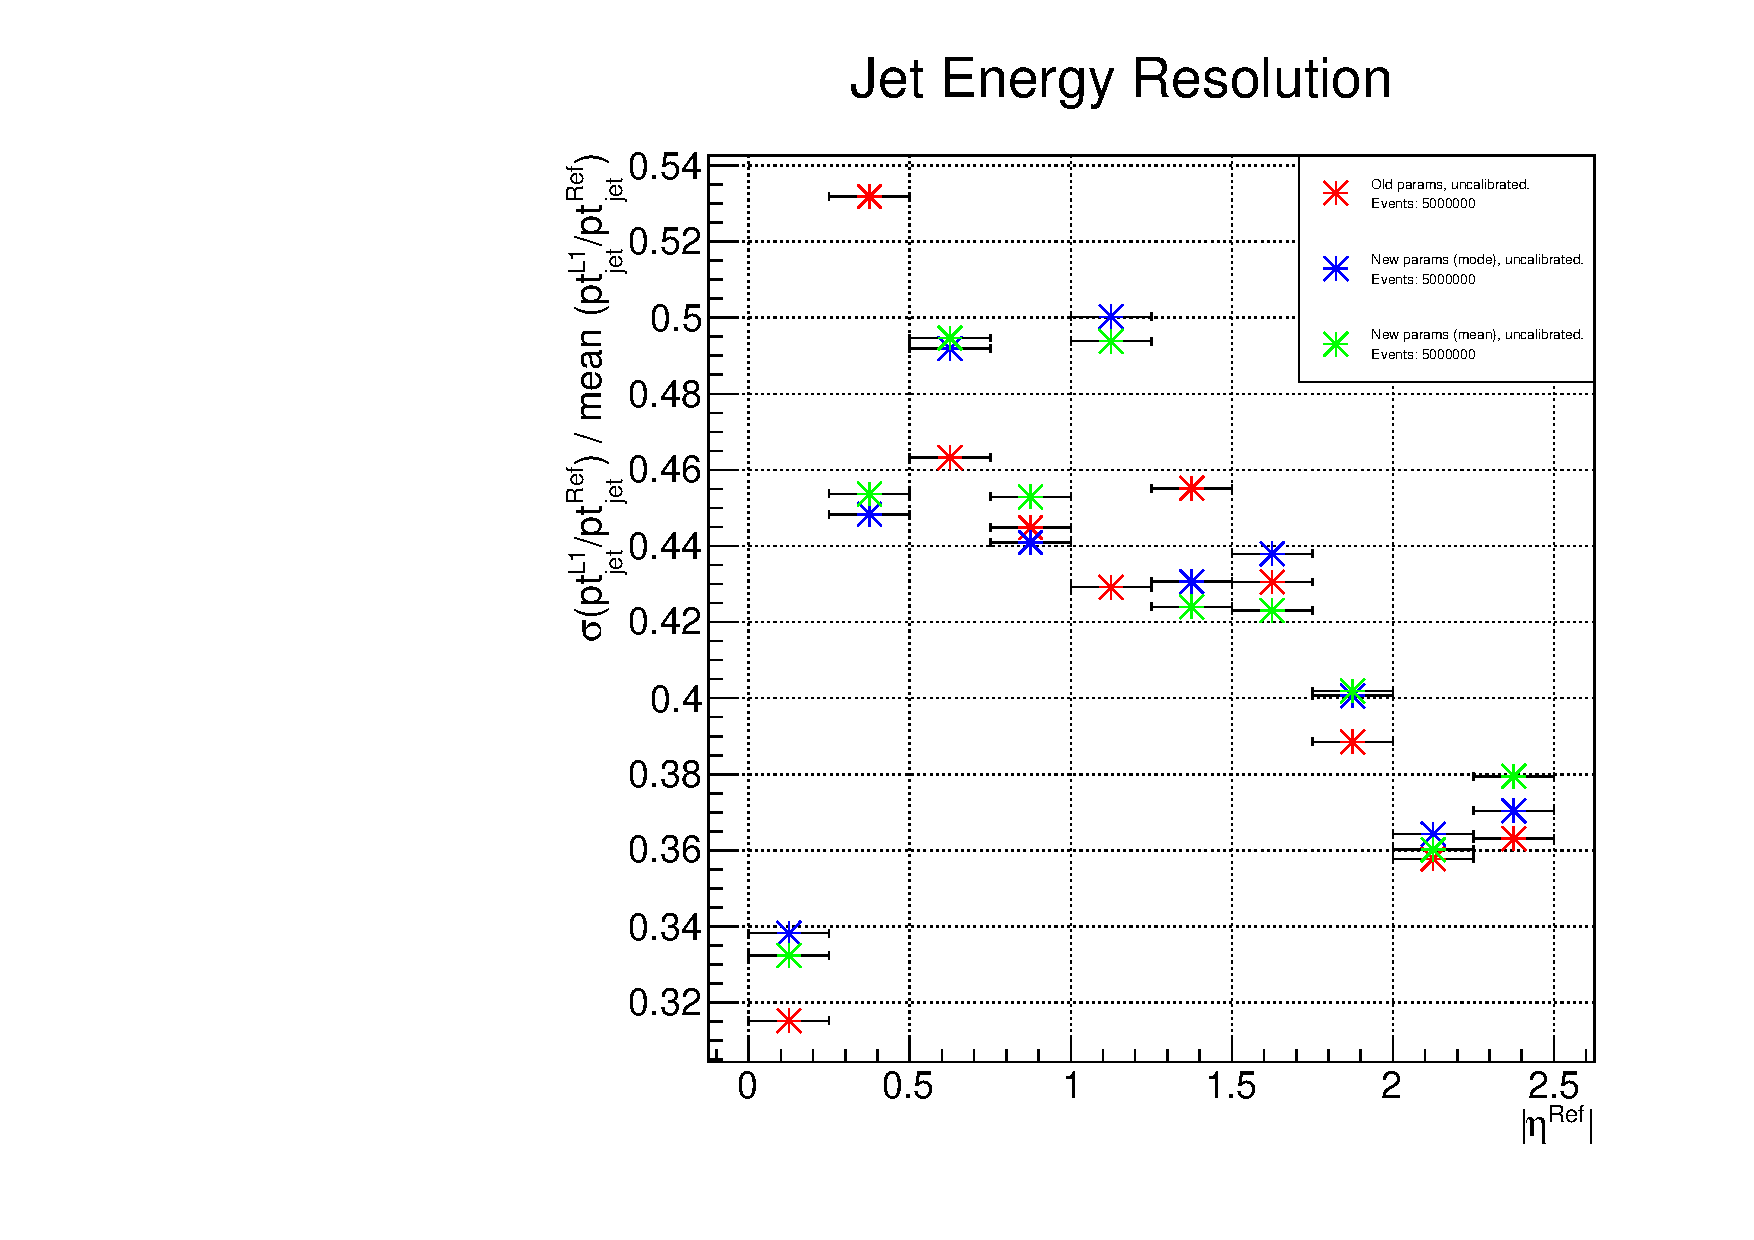
\includegraphics[width=110mm]{./sec20/jet_energy_resolution.pdf}
\caption{The jet energy resolution for the old params (red) and new params (blue) for different eta bins.}
\end{figure}


\section{CMS Week presentation on the Jet + MET status (05/12/2017)}

I've been asked to give a presentation during CMS Week about the 2017 status and 2018 plans of the jets and MET operations conducted by those in Calo Layer-2. The slides are linked here: \href{run:./sec20/20171205 L1 Jet + MET talk.pdf}{L1 Jet MET talk (05-12-2017).pdf}.


\section{Third round of JECs (end date -- 17/04/2018)}

As we've recently started the 2018 run of the LHC, we need calibrations to be conducted promptly so that the LUTs with scale factors can be deployed to the firmware, and data can be swiftly reconstructed and validated. The components I need are as follows:

\begin{easylist}
\easylistprops
& CMSSW version: 10.0.3
& Integration tag: \texttt{add100XLayer1SF} (encompasses tags \texttt{v97.20} - \texttt{97.22} rebased from CMSSW\_10\_0\_0)
& Dataset: /QCD\_Pt-15to3000\_TuneCP5\_Flat\_13TeV\_pythia8/RunIISpring18DR-NZSPU0to70\_100X\_upgrade2018\_realistic\_v10-v1/GEN-SIM-RAW
\end{easylist}

I could set up the environments in a similar way to before, but with some additions from various pull requests, bug fixes and rebases:

\begin{lstlisting}[belowskip=-0.7cm, language=sh, numbers=none]
cmsrel CMSSW_10_0_3
cd CMSSW_10_0_3/src
cmsenv
git cms-init
git cms-addpkg L1Trigger/Configuration
git cms-addpkg L1Trigger/L1TCalorimeter
git cms-addpkg L1Trigger/L1TCommon
git cms-addpkg L1Trigger/L1TMuon
git clone https://github.com/cms-l1t-offline/L1Trigger-L1TMuon.git L1Trigger/L1TMuon/data
git clone git@github.com:eshwen/L1JetEnergyCorrections.git L1Trigger/L1JetEnergyCorrections
git remote add bundocka git@github.com:bundocka/cmssw.git
git cms-merge-topic bundocka:add100XLayer1SF
git clone https://github.com/cms-l1t-offline/L1Trigger-L1TCalorimeter.git L1Trigger/L1TCalorimeter/data
scram b -j 8
\end{lstlisting}

I changed the jet calibration type in \textbf{caloParams\_2018\_v1\_1\_inconsistent\_cfi.py} and imported the file in \textbf{hackConditions\_cff.py}. Then, I navigated to \textbf{L1JetEnergyCorrections/python/} and used the \texttt{cmsDriver.py} command

\begin{lstlisting}[belowskip=-0.7cm, language=sh, numbers=none]
cmsDriver.py l1Ntuple -s RAW2DIGI --era=Run2_2018 --mc --python_filename=l1NtupleMcMaker2018_RAW2DIGI_v1.py --no_output -n 202 --conditions=100X_upgrade2018_realistic_v11 --customise=L1Trigger/Configuration/customiseReEmul.L1TReEmulMCFromRAWSimHcalTP --customise=L1Trigger/L1TNtuples/customiseL1Ntuple.L1NtupleRAWEMUGEN_MC --customise=L1Trigger/Configuration/customiseSettings.L1TSettingsToCaloParams_2018_v1_1_inconsistent --custom_conditions=HcalChannelQuality_2018_v3.0_mc,HcalChannelQualityRcd,frontier://FrontierProd/CMS_CONDITIONS --filein=/store/mc/RunIISpring18DR/QCD_Pt-15to3000_TuneCP5_Flat_13TeV_pythia8/GEN-SIM-RAW/NZSPU0to70_100X_upgrade2018_realistic_v10-v1/100000/00818B45-1522-E811-910B-1866DAEA7E64.root
\end{lstlisting}

to create the CMSSW config for the CRAB jobs. After testing with \texttt{cmsRun}, I then added the new dataset to \textbf{mc\_samples.py} and linked to it in \textbf{crab3\_stage2.py}, as well as updating \texttt{job\_append} and adding the CMSSW config to \texttt{PY\_CONFIG}. After initialising the CRAB environment, I submitted the initial ntuples with

\begin{lstlisting}[belowskip=-0.7cm, language=sh, numbers=none]
python crab3_stage2.py
\end{lstlisting}

I have also been asked to perform the JECs with ECAL zero suppression, which involved the same steps and workflow, but using the calo params file \textbf{caloParams\_2018\_v1\_1\_ECALZS\_inconsistent\_cfi.py}. The cmsDriver command was identical, apart from the output file name (in which I appended "ECAL\_ZS"), and the attribute of \texttt{L1Trigger/Configuration/customiseSettings} which I set to \texttt{L1TSettingsToCaloParams\_2018\_v1\_1\_ECALZS\_inconsistent}.

When tuning the fits for the curves made with the normal params, they were pretty terrible and wouldn't tune properly to capture the peak and tail of each curve. Joe suggested changing the values used in the fitting function in \textbf{runCalibration.py}. For a previous round of JECs (where the initial fits were decent), I found the root file and an accompanying LUT text file containing the parameters used in the fit. So I copied one of those lists and changed the one in the file to

\begin{lstlisting}[belowskip=-0.7cm, language=Python, numbers=none]
STAGE2_DEFAULT_PARAMS_JETMETERR = [1.86431, -1.34016e+06, -2.85506e-08, 20.2633, -6.40935e-07, -1.54, 1.06511]
\end{lstlisting}

Then, I reran \textbf{runCalibration.py} to get the root file with better fits I was able to tune. As with the CMSSW\_9\_2\_X JECs, I got the weird error \texttt{buffer is too small for requested array} when running \textbf{runCalibration.py}. Again, I had to source my CMSSW\_9\_0\_0\_pre2 release and run in that environment. I also had to apply another "Joe hack" for $2.964 < \abseta < 3.489$.

Once the calibrations were complete and the LUTs were made, I needed to perform the closure tests. To remake the ntuples with the calibrations, I needed to copy my \textbf{lut\_HR\_add\_mult.txt}, \textbf{lut\_HR\_pt.txt} and textbf{lut\_HR\_eta.txt} to \textbf{L1Trigger/L1TCalorimeter/data/} (giving the files some kind of unique marker to avoid confusion) and add the paths to those files in the calo params file. The variable \texttt{caloStage2Params.jetCalibrationLUTFile} requires the path to \textbf{lut\_HR\_add\_mult.txt}, then \texttt{jetCompressPtLUTFile} and \texttt{jetCompressEtaLUTFile} require the pt and eta LUTs, respectively. Then, I needed to change \texttt{jetCalibrationType} to turn the JECs on. The cmsDriver command was the same as when generating the config for the initial ntuples, just with a different \texttt{python\_filename}. The same recipe could be applied to JECs derived with the ECAL ZS params. I presented an update at the DPG meeting: \href{run:./sec20/20180423 L1 JEC comparison (2017 vs early 2018).pdf}{L1 JEC comparison (2017 vs early 2018).pdf}.


\subsection{Follow ups}

As outlined in the presentation, there was a problem with HF jet resolution among some other stuff. I was asked to make some scatter plots comparing different jet collections (GenJet vs offline CaloJet, Gen vs PFJet, PF vs Calo, PF vs L1Jet, and Calo vs L1Jet) in HF and in several $E_{\mathrm{T}}$ ranges. This was so we could get a rough idea of how these different offline or "true" measurements of jet \pt are related to each other and L1. Luckily, the L1JetEnergyCorrections repo has some support for this. In \textbf{submit\_matcher\_dag.py}, around L75, I could just change the \texttt{SAMPLE} variable and it would intelligently pick the correct C++ macro to run the matching out of the available options. And I could run it on the corrected or uncorrected ntuples.

When comparing PF and GenJets, I had to edit some of the code in \textbf{RunMatcherStage2PFGen.cpp}, replacing some out-of-date stuff and making it similar to \textbf{RunMatcherStage2L1Gen.cpp}. Namely, I had to update the names of the trees that house the properties of some of the collections and fix some variable names. Then, I had to write cpp files for each jet collection comparison in the same vein. All my edits will be in the commit logs for the repo. I also had to remember to compile everything after editing the C++ code and adding the new files to \textbf{BuildFile.xml} in the same directory, which also pointed out errors I needed to fix.

I could run the matcher like normal after the edit, as well as the calibration check (but making sure to rename the original pairs and checked root files so they weren't overwritten). Then, in \textbf{showoffPlots.py}, I just needed to make sure \texttt{l1\_str} and \texttt{ref\_str} matched the collections I was comparing. I could also set the $E_{\mathrm{T}}$ ranges in the relevant functions.

Originally, the PF and offline Calo objects (reco) weren't included in the ntuples, so Aaron remade them using the GEN-SIM-RAW and AOD formats of the QCD dataset.

\section{LHCP}

I was asked to present a poster at the LHC Physics (LHCP) conference in Bologna in June 2018. The poster title was titled "The CMS Level-1 jet and energy sum trigger for the LHC Run II". This mainly involved presenting the algorithms used for JetMET in Run-2 and the performance of the triggers in 2016 and 2017. My final version of the poster is linked here: \href{run:./sec20/LHCP poster JetMET 2018 v4.pdf}{LHCP poster JetMET 2018 v4.pdf}. After the conference, I submitted the poster to the proceedings.
